\section{Example}
\subsection{Cahn-Hilliard Equation}

%%%%%%%%%%%%%%%%%%%%%%%%%%%%%%%%%%%%%%%%%%%%%%%%%%%%%%%%%%%%%%%%%%%%%
\royslide{Free Energy Formulation}{

Cahn-Hilliard systems model material separation and interface
evolution based on a weakly non-local free energy density.

\begin{minipage}[h]{.55\textwidth}
\begin{eqnarray*}
f(c, \nabla c) & \equiv & f_0(c) + f_\gamma(\nabla c) \\
f_\gamma(\nabla c) & \equiv & \frac{\epsilon_c^2}{2} \nabla c \cdot \nabla c \\
%f_{0m}(c) & \equiv & \frac{1}{4} \left( c^2 - 1 \right)^2 \\
f_0(c) & \equiv & N k T \left( c \ln{(c)} + \right. \\
& & \left. (1-c) \ln{(1-c)} \right) + \\
& & N \omega c (1-c)
\end{eqnarray*}
\end{minipage}
\begin{minipage}[h]{.35\textwidth}
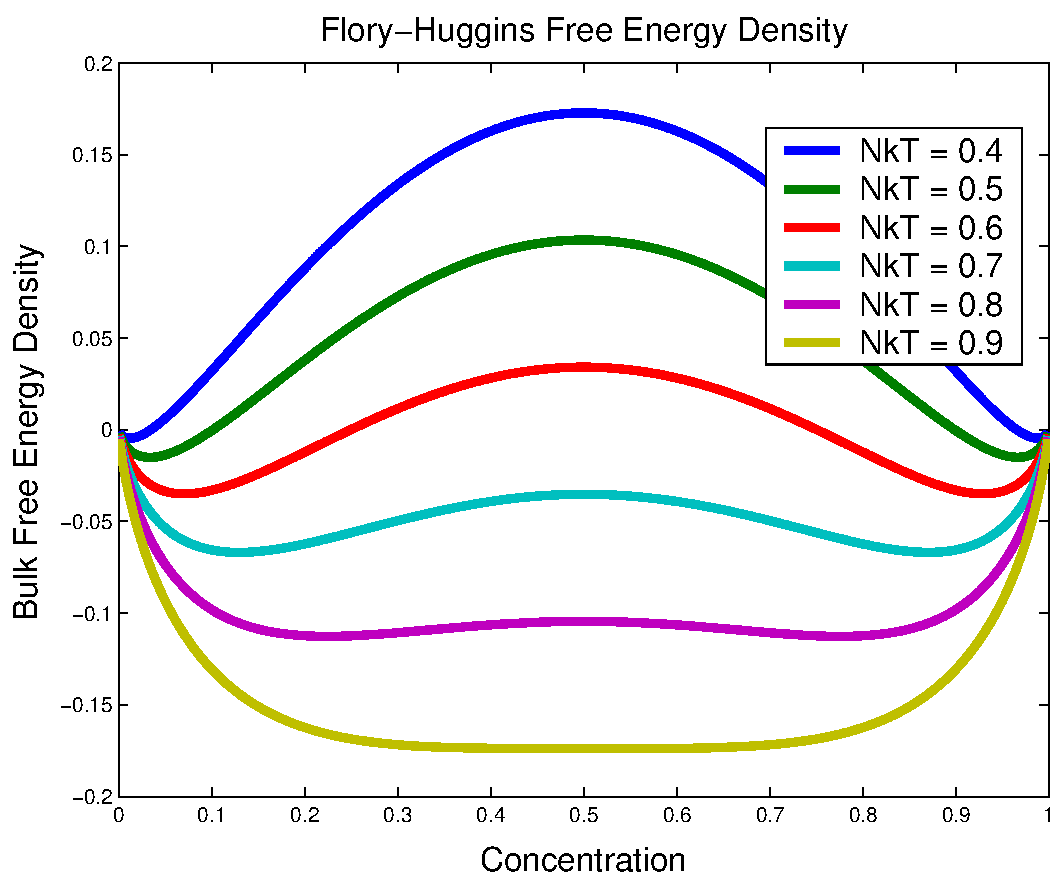
\includegraphics[width=.9\textwidth]{figs/energy}
\end{minipage}
}


%%%%%%%%%%%%%%%%%%%%%%%%%%%%%%%%%%%%%%%%%%%%%%%%%%%%%%%%%%%%%%%%%%%%%
\royslide{Cahn-Hilliard Equation}{

A mobility coefficient $M_c$ defines the concentration flux
$\vec{J}$.  For positive definite $M_c$, the resulting
Cahn-Hilliard equation gives globally non-increasing free energy.

\begin{eqnarray*}
\vec{J} & = & M_c \nabla \frac{df}{dc} 
  = M_c \nabla \left( f_0'(c) + f_\gamma'(c) \right)
\end{eqnarray*}
%\\
%f_{0m}' & = & c^3 - c \\
%f_{0c}' & = & N k T \left( \ln{(c)} - \ln{(1-c)} \right) + N \omega (1-2c) \\
%f_\gamma' & = & - \epsilon_c^2 \Laplacian c

\begin{eqnarray*}
\dt{c} & = & \nabla \cdot M_c \nabla
  \left( f_0'(c) - \epsilon_c^2 \Laplacian c \right)
\end{eqnarray*}

}


%%%%%%%%%%%%%%%%%%%%%%%%%%%%%%%%%%%%%%%%%%%%%%%%%%%%%%%%%%%%%%%%%%%%%
\royslide{Weak Cahn-Hilliard Equation}{

Taking a weighted residual and integrating by parts twice,

\begin{eqnarray*}
(\dt{c},\phi)_\Omega & = & - \left(M_c \nabla f_0'(c),
                \nabla \phi \right)_\Omega - \epsilon_c^2
                \left( \Laplacian c, \nabla \cdot M_c^T \nabla \phi
\right)_\Omega
\nonumber \\
  &   & + \left(\left(M_c \nabla \left( f_0'(c) -
          \epsilon_c^2 \Laplacian c\right) \right) \cdot \vec{n},
          \phi \right)_{\partial \Omega} \\
  &   & + \epsilon_c^2 \left( \Laplacian c, M_c^T \nabla \phi \cdot
\vec{n} \right)_{\partial \Omega}
\end{eqnarray*}

}


